\chapter{Placas, pines y cableado}\label{cap:placas}

\section{Vista general del cableado}

\begin{figure}[H]
\centering
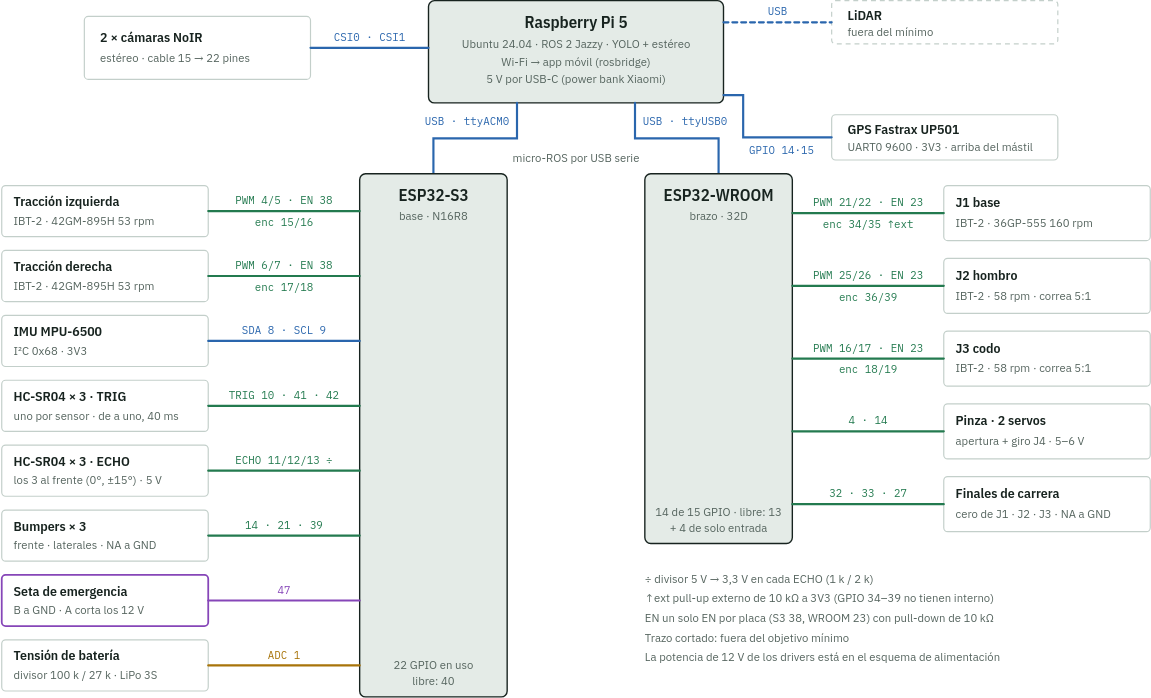
\includegraphics[width=\textwidth]{html_general.png}
\caption{Qué va conectado a qué, con el número de GPIO en cada cable (de \archivo{docs/html/conexiones.html}).
Azul: datos (USB, CSI, I²C, UART). Verde: GPIO y PWM. Ocre: analógico. Violeta: seguridad.}
\end{figure}

\begin{nota}[Dónde está la verdad]
Los pines \textbf{solo} se definen en \archivo{firmware/base/include/pins.h} y \archivo{firmware/brazo/include/pins.h}.
\archivo{docs/CONEXIONES.md} y las páginas de \archivo{docs/html/} los copian. Si hay una diferencia, manda
\cod{pins.h}. Las páginas HTML son interactivas: \archivo{docs/html/todo.html} junta todas, con cajas clickeables.
\end{nota}

\section{Tres ideas eléctricas que aparecen en todas partes}

\subsection{Los GPIO del ESP32 son de 3,3~V}
Un pin del ESP32 se rompe si recibe más de 3,6~V. Hay tres cosas en el robot que sacan 5~V: el ECHO de los HC-SR04,
los encoders de tracción y (si vuelve la 10S) la batería. Todas pasan por un \textbf{divisor resistivo}:
\[
V_\text{GPIO} = V_\text{entrada}\,\frac{R_\text{abajo}}{R_\text{arriba} + R_\text{abajo}}
\]
\begin{itemize}
  \item ECHO del HC-SR04: 1~kΩ arriba y 2~kΩ abajo: $5 \cdot \frac{2}{3} = 3{,}33$~V.
  \item Encoders de tracción: tienen un pull-up interno de 10~kΩ a 5~V; se agrega 20~kΩ a GND: $5 \cdot \frac{20}{30} = 3{,}33$~V.
  \item Batería: 100~kΩ arriba y 27~kΩ abajo: $12{,}6 \cdot \frac{27}{127} = 2{,}68$~V (el ADC lee hasta $\sim$3,1~V).
\end{itemize}

\subsection{Pull-up y pull-down}
Un pin de entrada ``al aire'' lee cualquier cosa. Un \textbf{pull-up} (resistencia a 3,3~V) lo deja en 1 cuando nada
lo conecta; el interruptor lo lleva a 0 conectándolo a GND. Así funcionan los bumpers, la seta y los finales de
carrera: \textbf{apretado = LOW}. El ESP32 tiene pull-ups internos, \textbf{salvo los GPIO 34 a 39 de la WROOM}, que
son solo de entrada y no tienen: ahí van los encoders, que traen su propio pull-up de 5,1~kΩ.

Un \textbf{pull-down} hace lo contrario. Los EN de los IBT-2 tienen uno de 10~kΩ: mientras el ESP32 arranca o se
reinicia, sus pines flotan; el pull-down mantiene los puentes deshabilitados y los motores quietos.

\subsection{La seta es normalmente cerrada (falla segura)}
El bloque B de la seta une el GPIO~47 con GND cuando está suelta. Al apretarla, o si \textbf{se corta un cable}, el pin
sube a HIGH por el pull-up y la S3 entra en EMERGENCIA. Un cable cortado se comporta como una seta apretada: es más
seguro que al revés.

\section{ESP32-S3: la base}

Placa Freenove ESP32-S3-WROOM N16R8, con USB nativo (aparece en la Pi como \cod{/dev/ttyACM0}). Va encima de una
\textbf{placa de expansión Freenove} con una bornera por pin, y los componentes (resistencias) van en dos perforadas
chicas, una sobre cada fila de borneras. Desde el 13/10 \textbf{no lleva capacitores}: bumpers y seta van directo.

{\small\begin{longtable}{@{}p{2.6cm} p{6.6cm} p{6.4cm}@{}}
\toprule
\textbf{GPIO} & \textbf{Conecta a} & \textbf{Nota} \\
\midrule
\endhead
4 · 5 & IBT-2 izquierdo RPWM · LPWM & PWM a 20~kHz, 10 bits \\
6 · 7 & IBT-2 derecho RPWM · LPWM & 20~kHz \\
38 & R\_EN + L\_EN de los dos IBT-2 & pull-down 10~kΩ \\
15 · 16 & Encoder izquierdo A · B & amarillo · blanco; 20~kΩ a GND \\
17 · 18 & Encoder derecho A · B & amarillo · blanco; 20~kΩ a GND \\
8 · 9 & IMU SDA · SCL & I²C 400~kHz, dirección 0x68 \\
10 · 41 · 42 & TRIG del HC-SR04 frente · izquierda · derecha & disparados de a uno, cada 40~ms \\
11 · 12 · 13 & ECHO frente · izquierda · derecha & divisor 1~k / 2~k \\
14 · 21 · 39 & Bumpers frente · izquierda · derecha & NA a GND, pull-up interno \\
47 & Seta, bloque B (NC) & a GND; HIGH = apretada o cable cortado \\
1 & Divisor de batería 100~k / 27~k & ADC1 canal 0 \\
40 & libre & reservado para un 4.º bumper \\
\bottomrule
\end{longtable}}

Prohibidos en la S3: 19/20 (USB), 26--37 (memoria flash y PSRAM). Evitar: 0/3/45/46 (\textit{strapping}: definen el
modo de arranque), 43/44 (UART0), 2/48 (LED).

\begin{pendiente}[LED RGB de la S3]
En la DevKitC-1 v1.1 el LED RGB está en el GPIO~38, que es el EN de la tracción. \cod{pins.h} supone el 48. Verificar
la placa real y no usar nunca el LED RGB en el firmware.
\end{pendiente}

\begin{figure}[H]
\centering
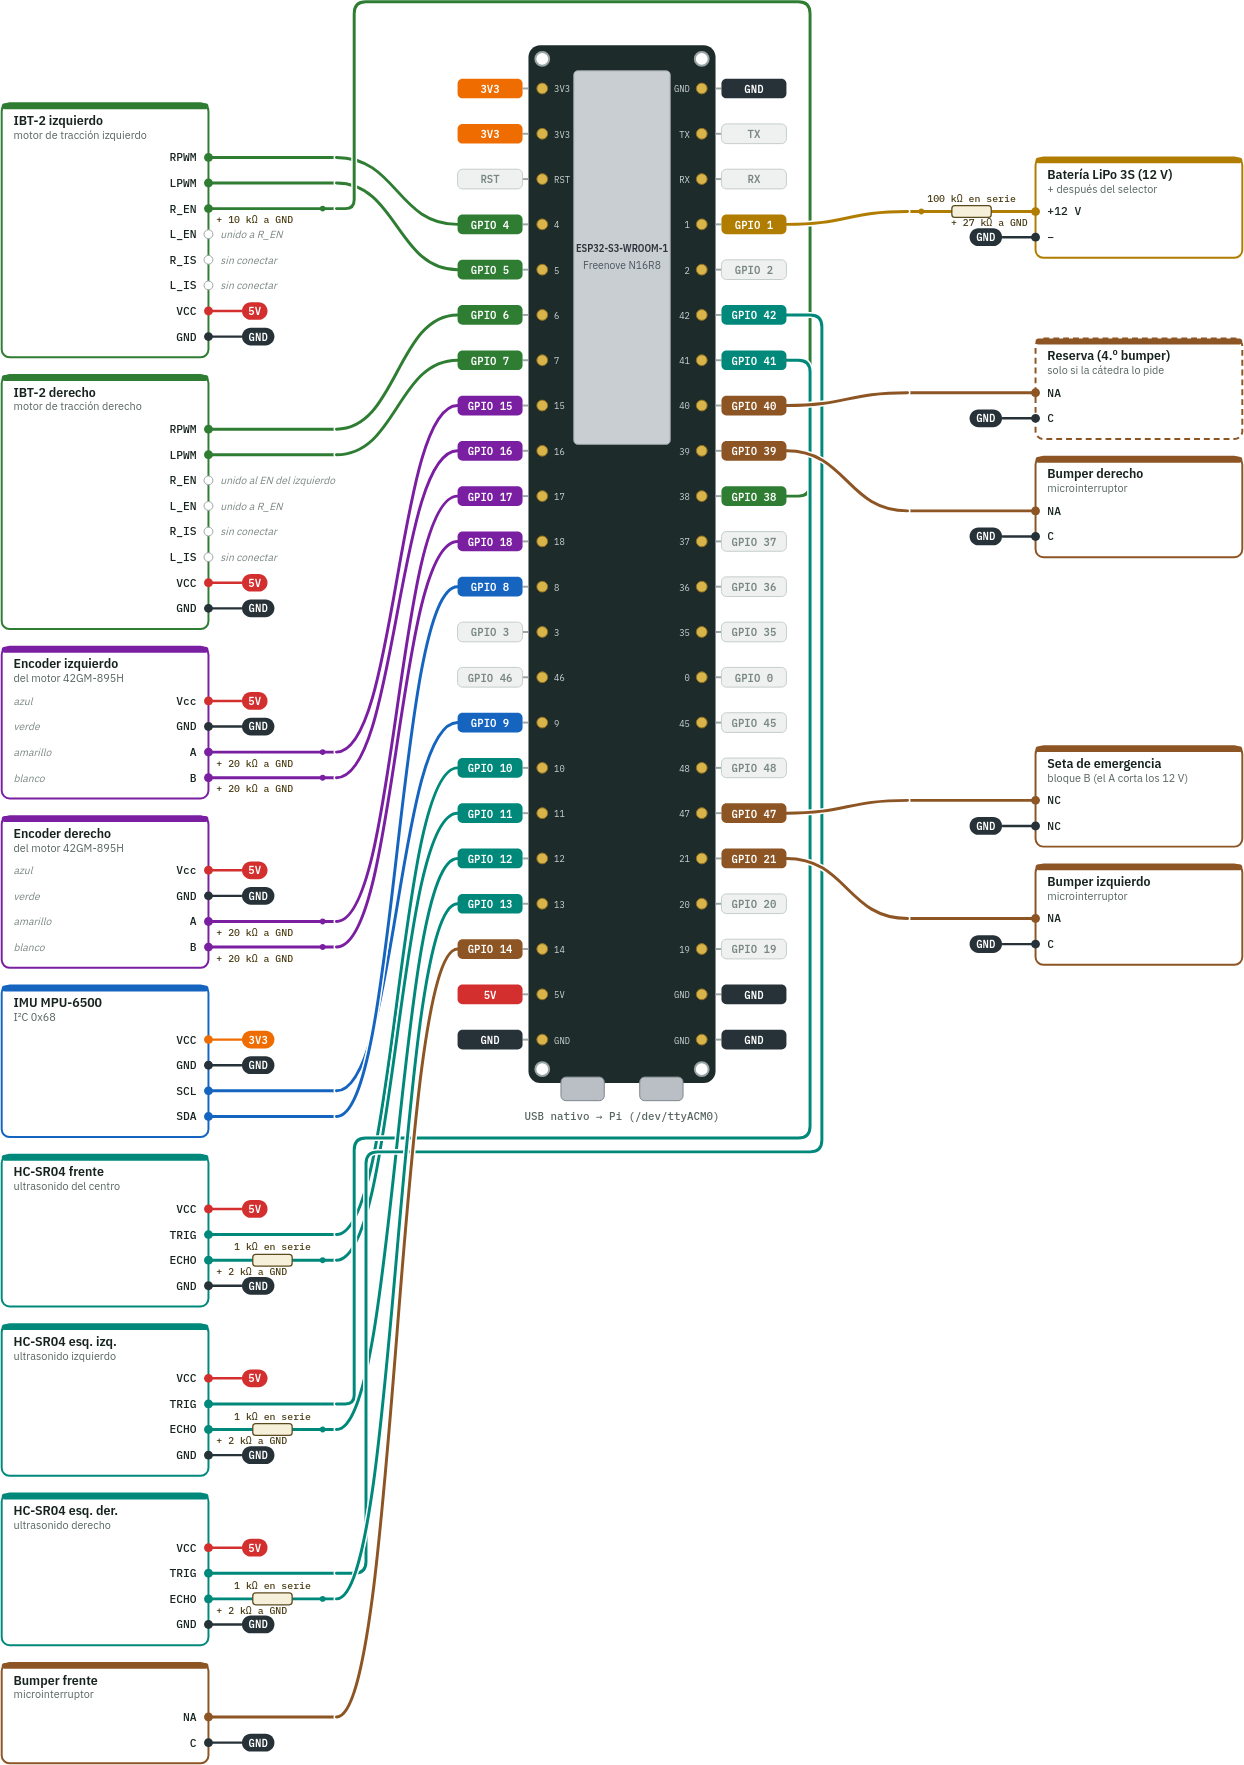
\includegraphics[height=0.82\textheight]{html_s3_cableado.png}
\caption{Cableado de la S3: cada periférico a un costado, con un cable de color de cada pin al pin de la ESP32
(de \archivo{docs/html/placa\_s3.html}). Las resistencias se dibujan sobre el cable.}
\end{figure}

\begin{figure}[H]
\centering
\begin{subfigure}{0.58\textwidth}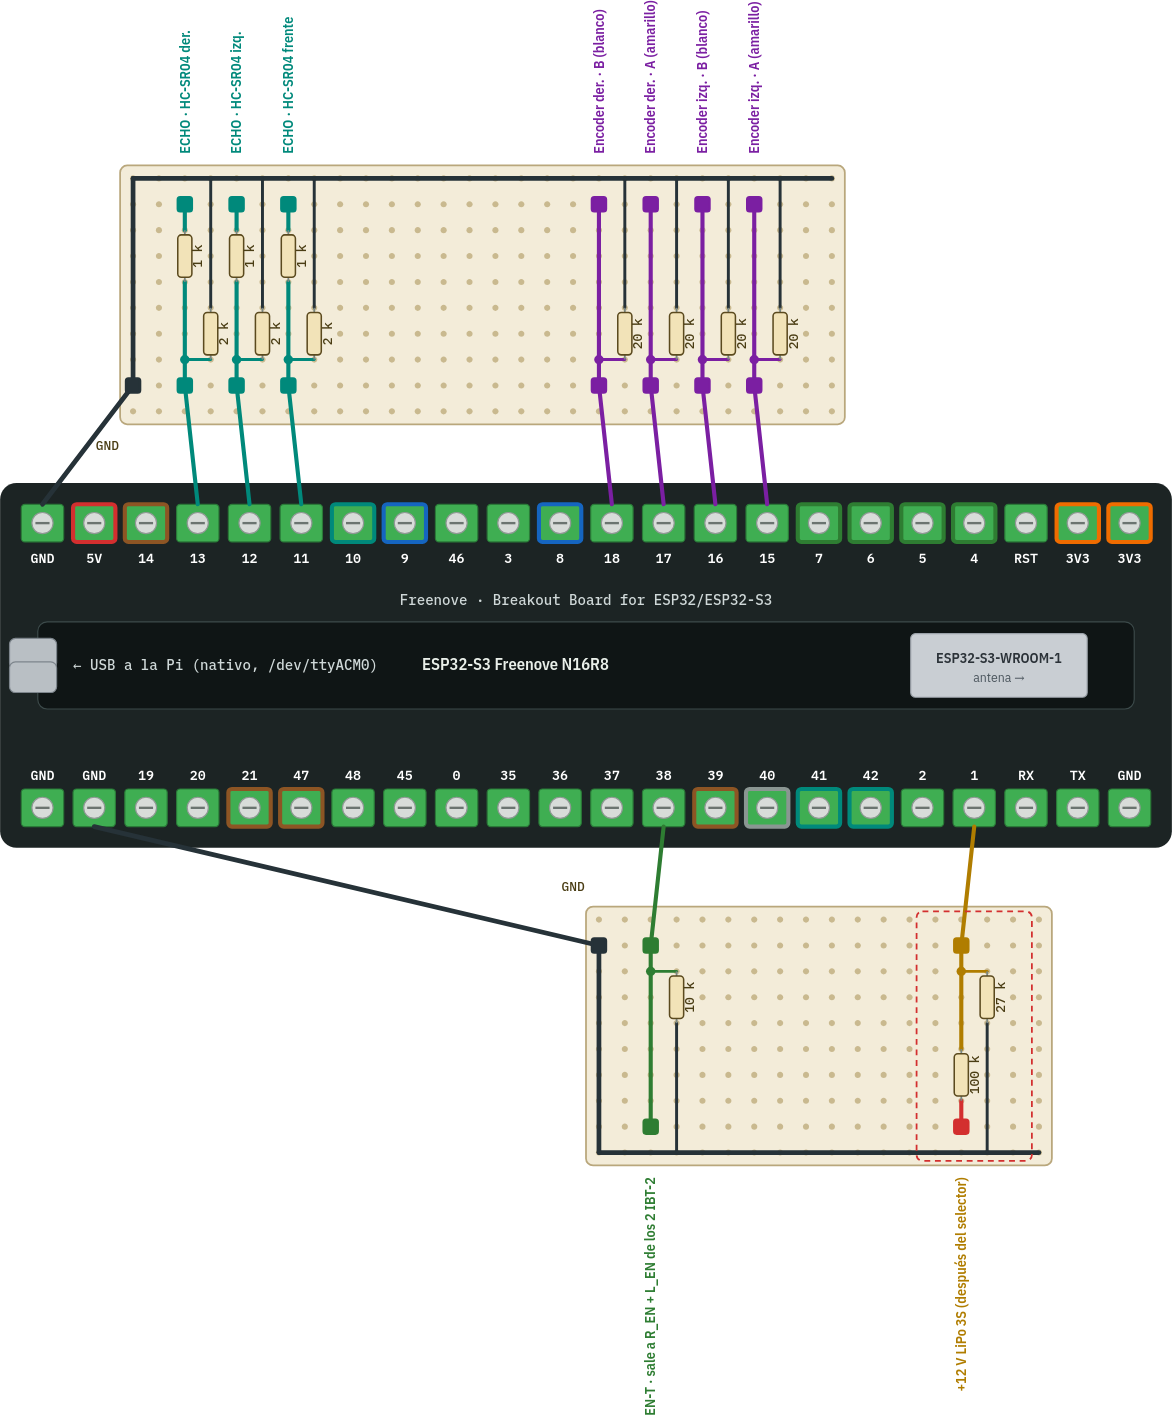
\includegraphics[width=\linewidth]{html_s3_perforadas.png}\caption{La Freenove con las dos perforadas.}\end{subfigure}\hfill
\begin{subfigure}{0.38\textwidth}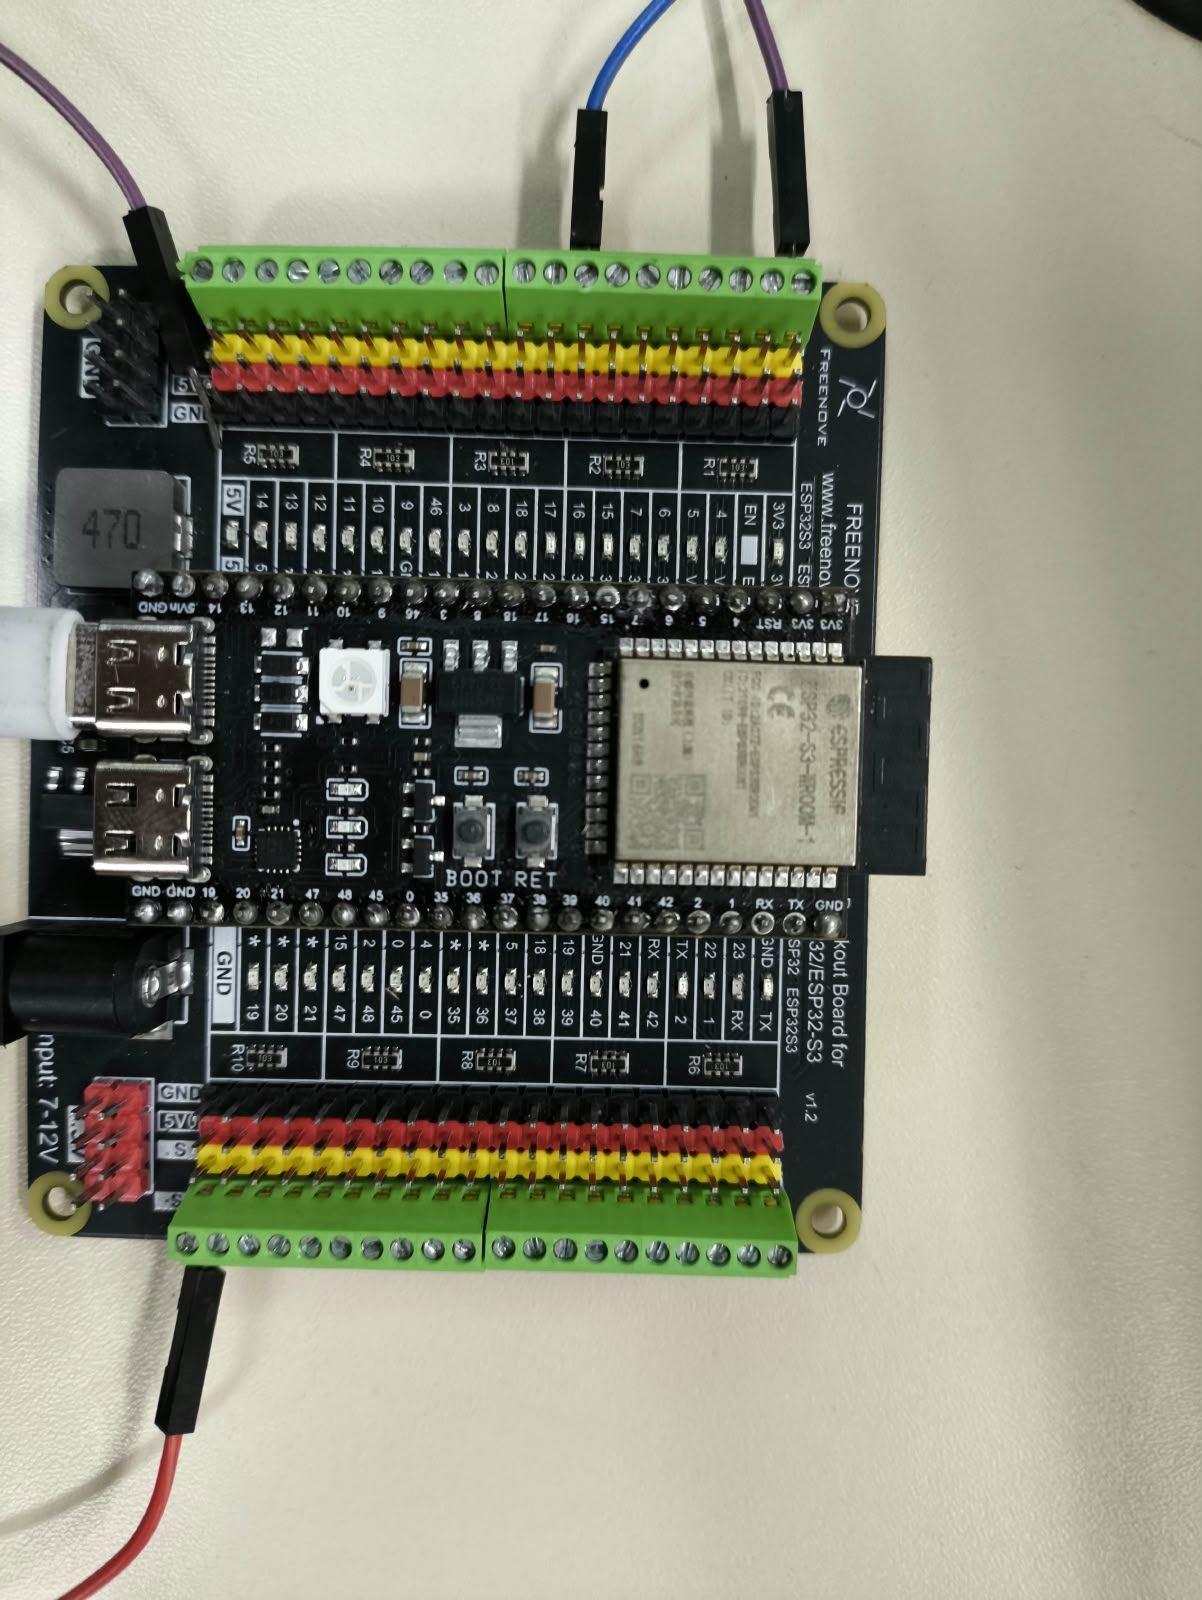
\includegraphics[width=\linewidth]{s3_foto.jpg}\\[4pt]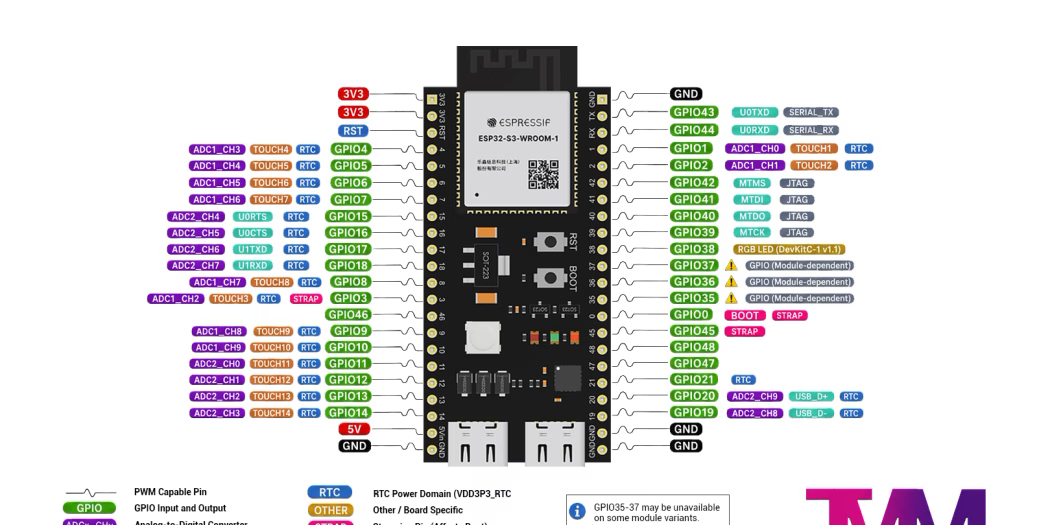
\includegraphics[width=\linewidth]{pinout_s3.png}\caption{Placa real y pinout.}\end{subfigure}
\caption{Montaje de la S3.}
\end{figure}

\section{ESP32-WROOM-32D: el brazo}

Placa HW-394 de 30 pines (USB-C, conversor CH340: aparece como \cod{/dev/ttyUSB0}), enchufada en un \textbf{shield de
borneras}, más una perforada chica de distribución con rieles de 5~V, 3,3~V, EN, GND y 6~V. Pines v0.5 (12/10).

{\small\begin{longtable}{@{}p{2.6cm} p{6.6cm} p{6.4cm}@{}}
\toprule
\textbf{GPIO} & \textbf{Conecta a} & \textbf{Nota} \\
\midrule
\endhead
21 · 22 & J1 IBT-2 RPWM · LPWM & 20~kHz (probado) \\
25 · 26 & J2 IBT-2 RPWM · LPWM & \\
16 · 17 & J3 IBT-2 RPWM · LPWM & \\
23 & R\_EN + L\_EN de los 3 IBT-2 & pull-down 10~kΩ (la única resistencia) \\
34 · 35 & Encoder J1 A · B & solo entrada; pull-up de la placa del encoder \\
36 (VP) · 39 (VN) & Encoder J2 A · B & solo entrada; pull-up de la placa del encoder \\
18 · 19 & Encoder J3 A · B & \\
4 & Servo de apertura & 50~Hz \\
14 & Servo de giro (J4) & saca pulsos al arrancar: el servo puede moverse un instante \\
32 · 33 · 27 & Finales de carrera J1 · J2 · J3 & NA a GND, pull-up interno \\
13 & libre & reserva \\
\bottomrule
\end{longtable}}

Evitar en la WROOM: 6--11 (flash), 0/2/5/12/15 (\textit{strapping}), 1/3 (UART0 = USB).

\begin{nota}[Un solo EN para las tres articulaciones]
Los tres IBT-2 del brazo comparten el EN (GPIO~23). Consecuencia: no se puede dejar una articulación en rueda libre
mientras otra se mueve. La que no se mueve queda \textbf{frenada} (puente habilitado con PWM 0). Rueda libre solo
cuando las tres están libres.
\end{nota}

\begin{figure}[H]
\centering
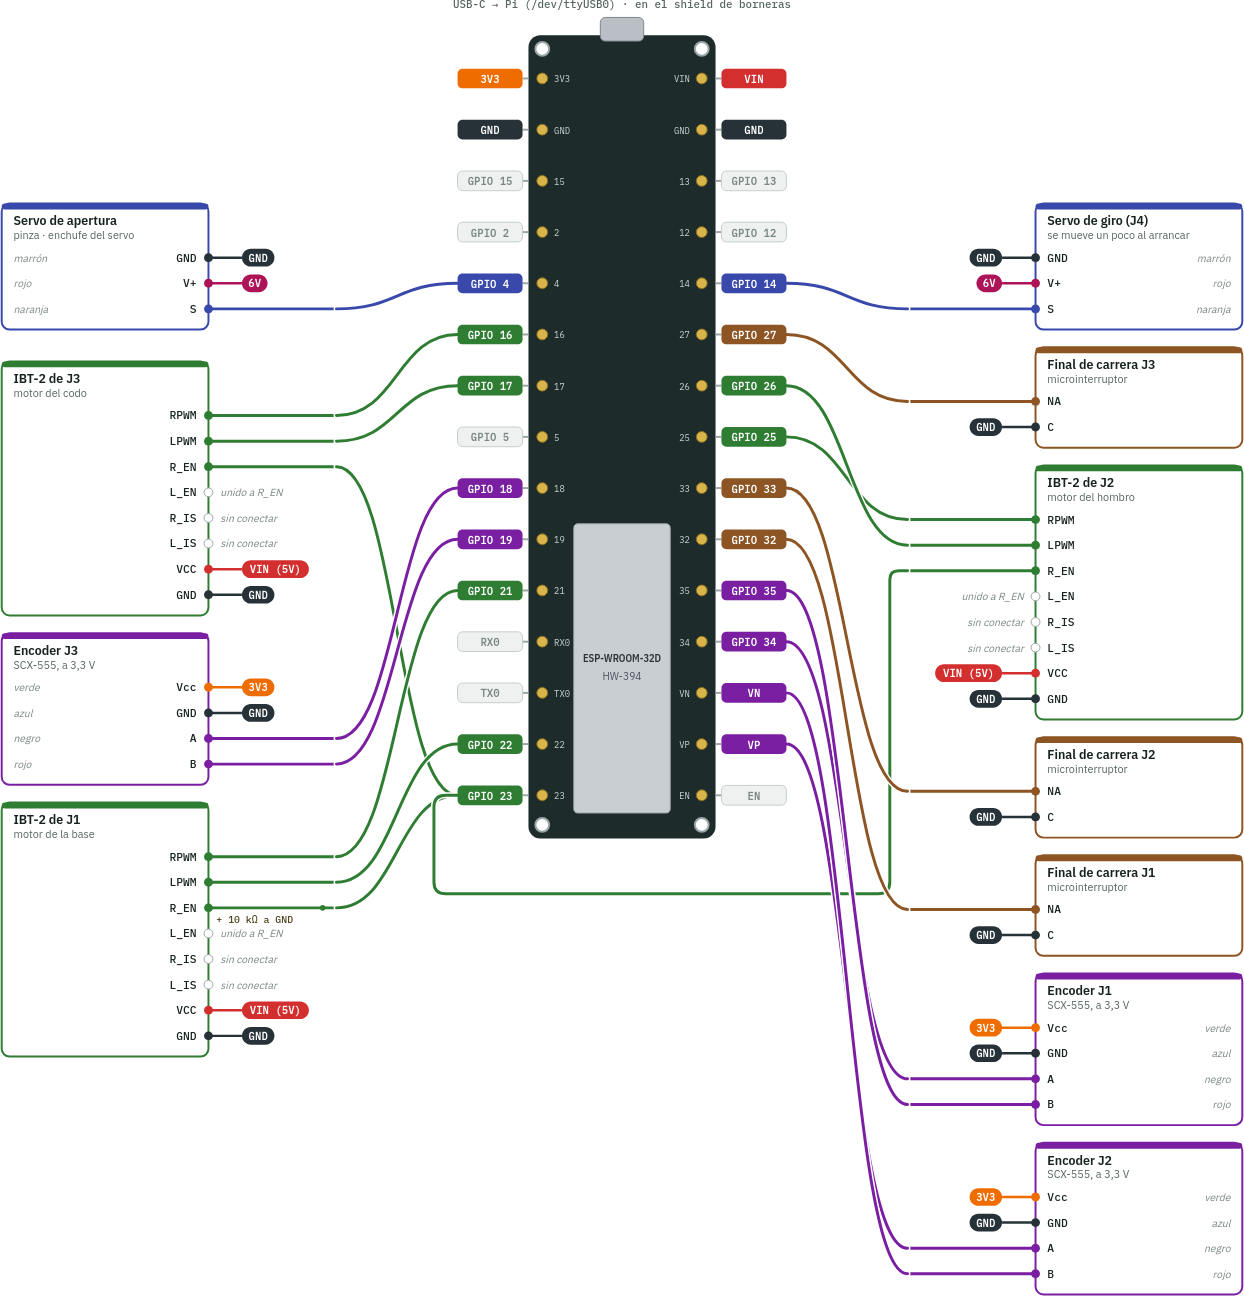
\includegraphics[width=\textwidth]{html_wroom_cableado.png}
\caption{Cableado de la WROOM (de \archivo{docs/html/placa\_wroom.html}).}
\end{figure}

\begin{figure}[H]
\centering
\begin{subfigure}{0.62\textwidth}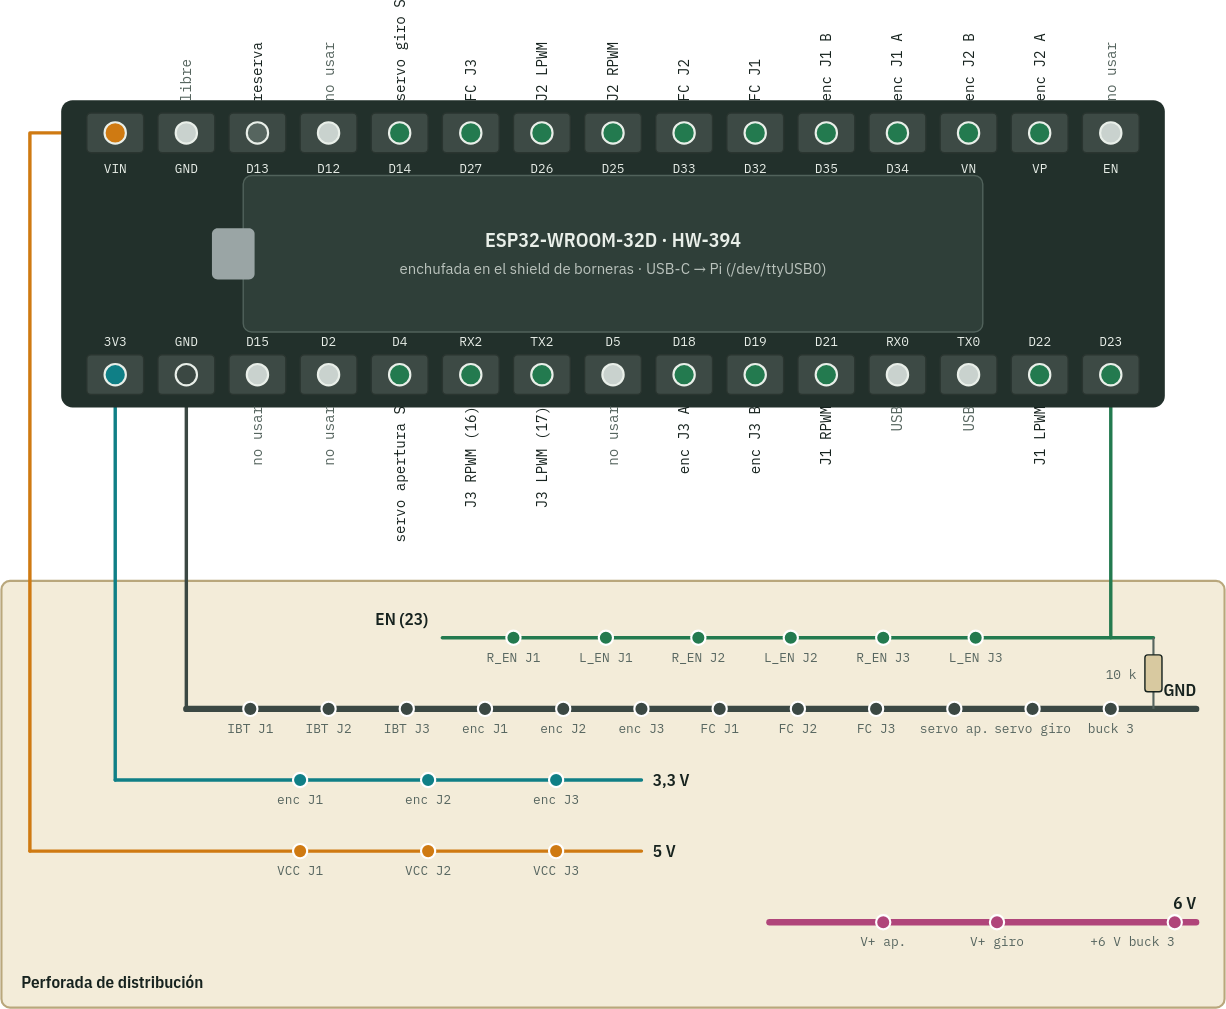
\includegraphics[width=\linewidth]{html_wroom_plano.png}\caption{Shield y perforada de distribución.}\end{subfigure}\hfill
\begin{subfigure}{0.34\textwidth}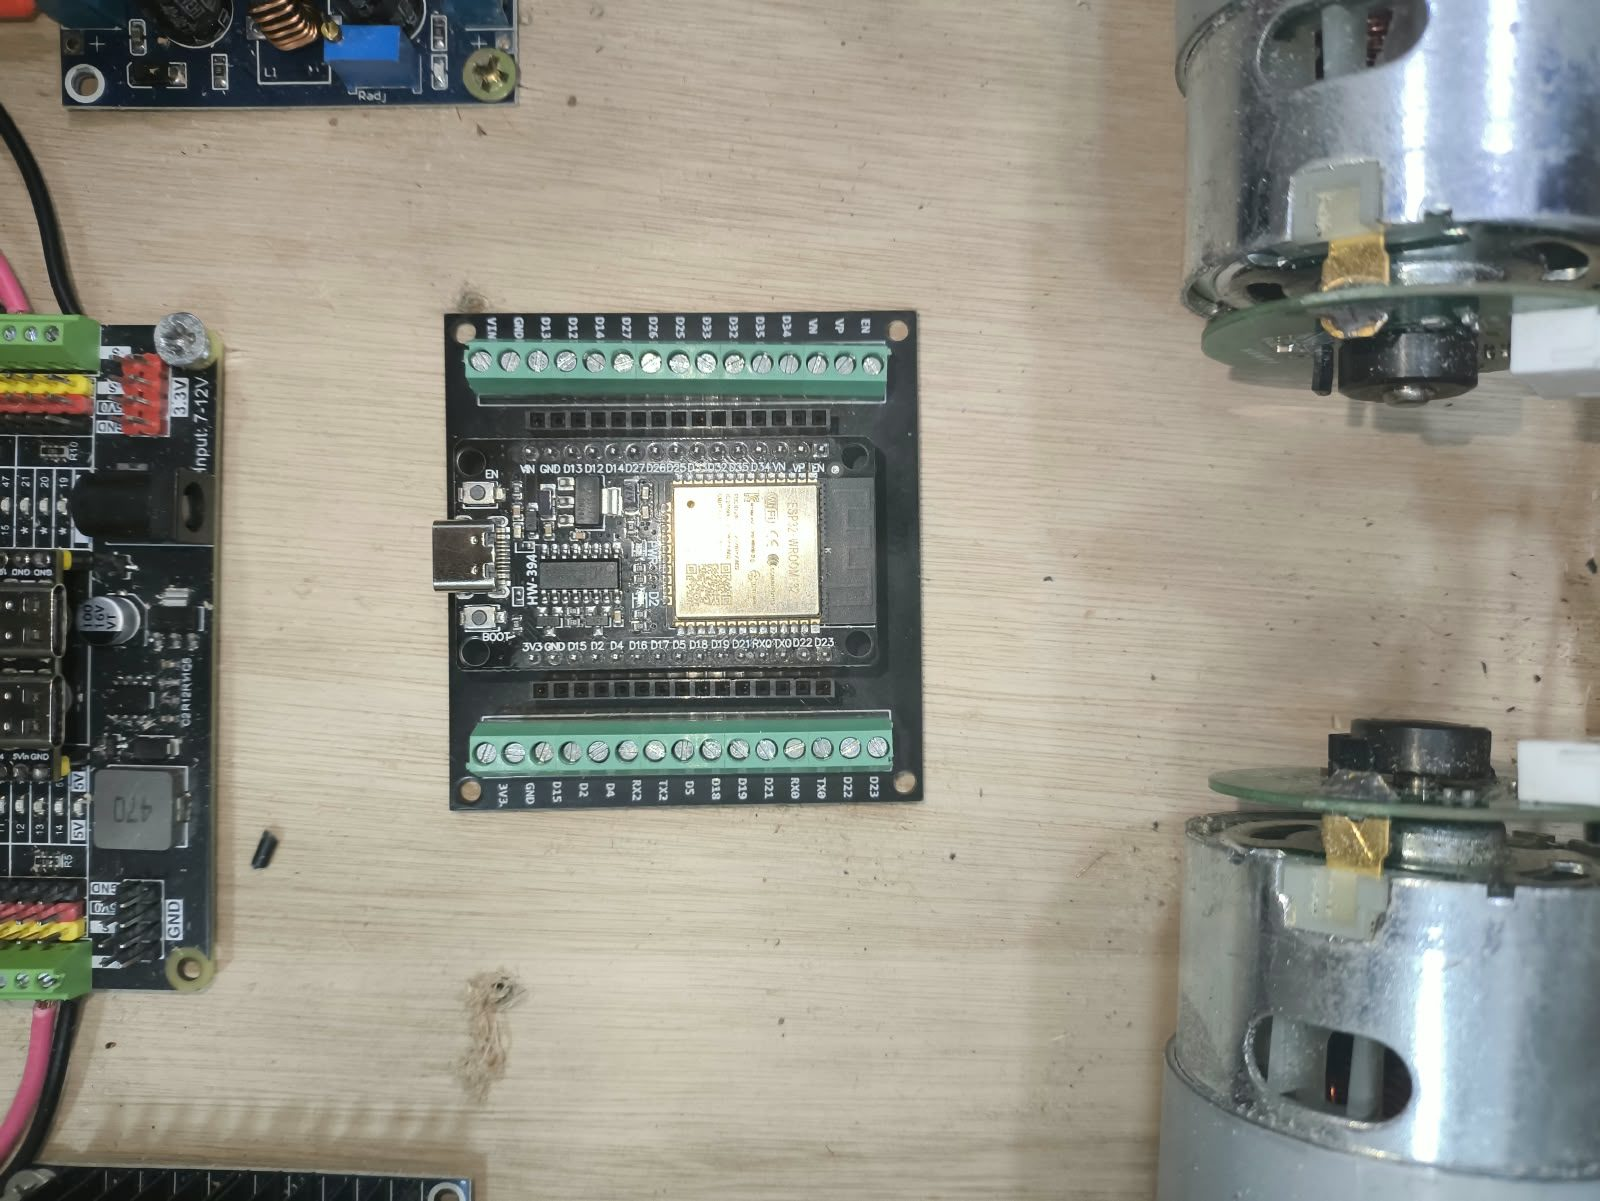
\includegraphics[width=\linewidth]{shield_wroom.jpg}\caption{Shield de borneras real.}\end{subfigure}
\caption{Montaje de la WROOM.}
\end{figure}

\section{Raspberry Pi 5}

{\small
\begin{tabularx}{\textwidth}{@{}l l X@{}}
\toprule
\textbf{Puerto} & \textbf{Conecta a} & \textbf{Nota} \\
\midrule
CSI0 · CSI1 & Cámaras NoIR izquierda · derecha & cable plano de 15 a 22 pines \\
USB & ESP32-S3 (base) & micro-ROS (\cod{/dev/serial/by-id/}\ldots) \\
USB & ESP32-WROOM (brazo) & micro-ROS a 115\,200 baudios \\
GPIO 14 · 15 (pines 8 · 10) & GPS UP501: RX · TX del GPS & UART0, \cod{/dev/ttyAMA0}, 9600 baudios, 3,3~V \\
USB-C & Power bank & 5~V 3~A \\
\bottomrule
\end{tabularx}}

La Pi va \textbf{arriba del mástil, junto a las cámaras}: el cable CSI es corto y sensible a interferencias, mientras
que el USB aguanta 1--2~m. Bajan por el mástil los dos USB hacia los ESP32. Los GPIO se atornillan en un HAT pasivo
de borneras.

\begin{nota}[Por qué usar \cod{/dev/serial/by-id/}]
Los nombres \cod{/dev/ttyACM0} y \cod{/dev/ttyUSB0} pueden cambiar (la S3 pasa a veces de ACM0 a ACM1 al reiniciarse).
Los enlaces de \cod{/dev/serial/by-id/} tienen el nombre del fabricante y no cambian: usarlos en los agentes.
\end{nota}

\begin{nota}[Corriente de los USB]
Sin la fuente oficial de 5~A, la Pi limita a 600~mA el total de los USB \textbf{y el ventilador}. Alcanza para los dos
ESP32 (unos 400~mA con sensores). No activar \cod{usb\_max\_current\_enable=1}. Verificar con la visión corriendo
10~min: \cod{vcgencmd get\_throttled} tiene que dar \cod{0x0}.
\end{nota}

\section{La seta, cable por cable}

\begin{figure}[H]
\centering
\begin{subfigure}{0.40\textwidth}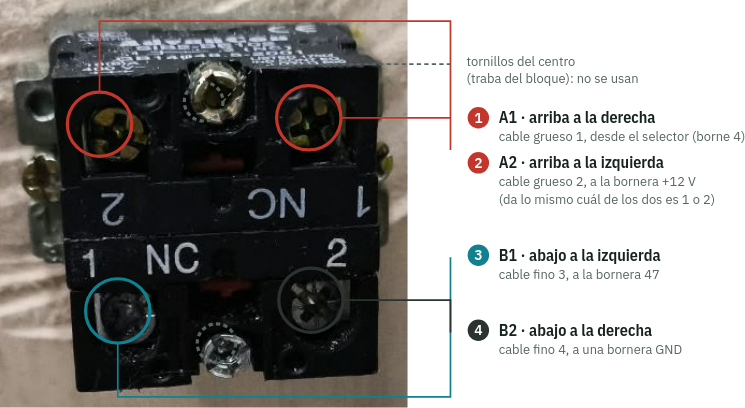
\includegraphics[width=\linewidth]{html_seta_foto.png}\caption{Qué tornillo es cuál.}\end{subfigure}\hfill
\begin{subfigure}{0.56\textwidth}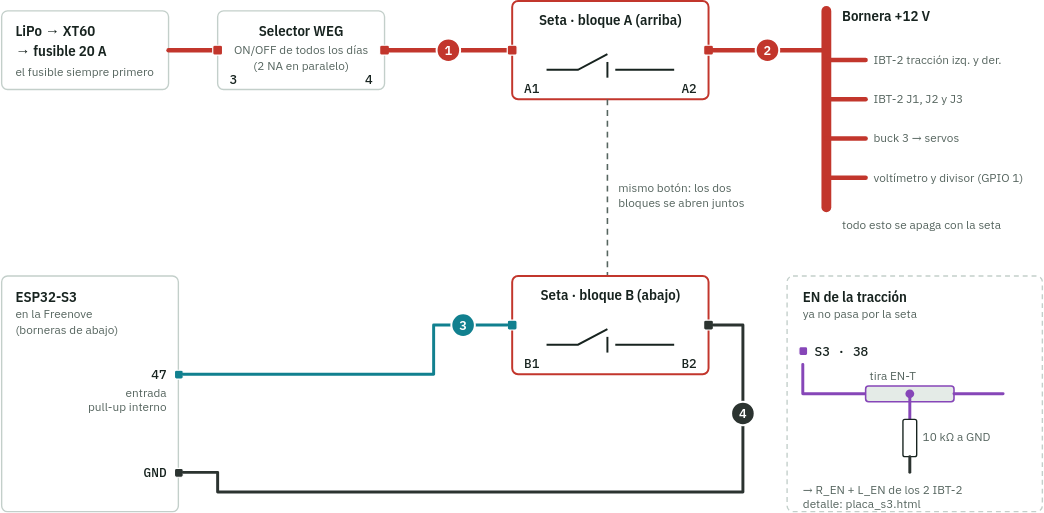
\includegraphics[width=\linewidth]{html_seta_circuito.png}\caption{Los 4 cables.}\end{subfigure}
\caption{La seta (de \archivo{docs/html/seta.html}). Bloque A (arriba): cables 1 y 2, en el + del bus de 12~V.
Bloque B (abajo): cables 3 y 4, entre el GPIO~47 y GND.}
\end{figure}

Antes de cablearla, \textbf{probar con el multímetro qué contactos son NC}. Prueba: con la seta apretada, 0~V en la
bornera +12~V y \cod{armar} tiene que fallar; al soltarla, las ruedas no arrancan solas.
